\documentclass{article}
%\usepackage{harvard}
\usepackage[english]{babel}

% Set page size and margins
\usepackage[a4paper,top=2cm,bottom=2cm,left=3cm,right=3cm,marginparwidth=1.75cm]{geometry}

% Useful packages
\usepackage{amsmath}
\usepackage{graphicx}
\usepackage[colorlinks=true, allcolors=blue]{hyperref}
\usepackage{amsfonts} 


\title{Neural architecture search with target hardware control}
\author{Firsov Sergey\\
        Intelligent Systems Phystech}

\begin{document}
\maketitle

\begin{abstract}
The paper examines the problem of deep learning model selection with respect to target hardware. We introduce a novel neural architecture search (NAS) method that simultaneously considers model accuracy, complexity, and hardware efficiency. The complexity of the model is measured by the number of parameters, while the hardware constraints are represented by the overall latency of network operations on the target device. Our approach builds upon Differentiable Architecture Search (DARTS), treating network structural parameters as functions of a complexity parameter, and extends it by incorporating latency-aware optimization inspired by FBNet.

Specifically, we propose replacing the scalar complexity parameter with a simplex-based complexity vector, allowing finer and more granular control over the inclusion of various operations. By integrating latency estimation through differentiable latency-aware optimization, and introducing Gumbel-Softmax sampling together with hypernetworks, our method enables simultaneous optimization of multiple architectures across a range of complexity levels. This unified optimization procedure generates a family of architectures tailored to different computational budgets within a single training process, significantly reducing search time and resources.
% The paper examines the problem of deep learning model selection with respect to target hardware. We introduce a novel neural architecture search (NAS) method that simultaneously considers model accuracy, complexity, and hardware efficiency. The complexity of the model is measured by the number of parameters, while the hardware constraints are represented by the overall latency of network operations on the target device. 

% This approach builds upon Differentiable Architecture Search (DARTS), treating network structural parameters as functions of a complexity parameter, and extends it by incorporating latency-aware optimization inspired by FBNet. By introducing Gumbel-Softmax sampling and hypernetworks, we enable simultaneous optimization of multiple architectures across a range of complexity levels. This results in a single optimization process that identifies a family of architectures tailored to different computational budgets, reducing search time and resources.
\end{abstract}

\section{Introduction}

Selecting an appropriate architecture for deep learning models is a crucial task that directly impacts model efficiency and performance. With deep learning continuing to push computational limits, researchers face the challenge of finding a balance between model complexity, accuracy, and resource consumption. Recent advances in Neural Architecture Search (NAS) techniques ~\cite{nas}, such as Differentiable Architecture Search (DARTS)~\cite{liu2019darts}, seek to automate this process by exploring large search spaces of possible network structures. However, these methods often struggle with high computational requirements and the need for architecture adjustments when model complexity or target hardware changes~\cite{yakovlev2021neural}. % ~\cite{Wu_2019_CVPR},

One of the significant developments in NAS is the introduction of hardware-aware models. For example, FBNet~\cite{Wu_2019_CVPR} incorporates latency into the architecture search process, optimizing not only model performance but also hardware efficiency. This approach addresses the mismatch between FLOPs and actual hardware performance, a limitation of many prior NAS methods. FBNet achieves this through gradient-based optimization and Gumbel-Softmax sampling, which dramatically reduce the search costs while generating a family of hardware-optimized models.
% MnasNet

Similar ideas are used in ProxylessNAS~\cite{proxylessnas}, which solves the problem of high memory and computing costs by optimizing architectures directly on large tasks and target hardware platforms, without using proxy tasks. ProxylessNAS introduces a direct search engine (Reinforce sampling) for learning architectures on large datasets and simulates operation delays to account for hardware limitations. However, this approach requires careful calibration, as enhanced learning often suffers from high variance.

Building on these ideas, our work improves upon DARTS-CC~\cite{yakovlev2021neural} %тут как будто переделать надо
, a NAS approach that uses hypernetworks to control model complexity during architecture search. Unlike other methods that search for individual architectures at different complexity levels, DARTS-CC generates multiple architectures in a single optimization process. Inspired by FBNet, we extend DARTS-CC by integrating latency-aware optimization and replacing the scalar complexity parameter with a simplex-based representation of architecture choices. This enables simultaneous search for architectures optimized across multiple complexity and latency levels, further reducing NAS time, and ensuring deployability across diverse hardware environments.

% Это уже наверное в метод идёт или в заключение
% Our contributions can be summarized as follows:  
% \begin{itemize}
%     \item We extend DARTS-CC by incorporating hardware latency into the optimization process. This enables the discovery of architectures that are not only accurate, but also efficient on target devices.
%     \item We replace the scalar complexity parameter in DARTS-CC with a simplex-based representation, allowing the use of Gumbel-Softmax sampling for flexible architecture optimization.
%     \item We propose a unified framework that combines latency-aware optimization, hypernetworks, and Gumbel-Softmax sampling to generate a family of architectures in a single optimization run.
%     \item We validate our method on multiple datasets and hardware platforms, demonstrating improved efficiency and flexibility compared to existing NAS approaches.
% \end{itemize}

%%%%%%%%%%%%%%%%%%%%%%%%%%
\subsection{Proposed Method}
The proposed method formulates Neural Architecture Search (NAS) as an optimization problem that simultaneously considers model accuracy, complexity, and hardware efficiency.  % мне тут не хватает ещё текста описания

\textbf{Problem Formulation.} In conventional DARTS the goal is to find architectural parameters \(\boldsymbol{\alpha} \in \mathcal{A}\) and model weights \(\boldsymbol{w} \in \mathcal{W}\) such that the loss function \(L(\boldsymbol{w}, \boldsymbol{\alpha})\) is minimized. The optimization problem can be formulated as follows:

\[
\min_{\boldsymbol{\alpha} \in \mathcal{A}} \big[L(\boldsymbol{w}^*(\boldsymbol{\alpha}), \boldsymbol{\alpha}) \big],
\]

where \(L(\boldsymbol{w}, \boldsymbol{\alpha})\) represents the task loss.  \\
However, DARTS does not account for flexibility in controlling model complexity or hardware constraints. So we propose these extensions to the DARTS framework to address its limitations:


\subsection{Architecture Representation}

We define the architectural parameters $\boldsymbol{\alpha}$ as a function of a complexity vector $\boldsymbol{S}$, which belongs to a $(k-1)$-dimensional simplex:

$$
\boldsymbol{S} \in \Delta^{k-1} = \left\{ \boldsymbol{S} \in \mathbb{R}^{k} \mid \sum_{i=1}^{k} S_i = 1,\, S_i \geq 0 \right\},
$$

where $k$ is the number of possible operation types. Each component $S_i$ represents the relative importance or penalization of the $i$-th operation type, thus enabling more granular and precise control over architecture complexity and the inclusion or exclusion of specific operations.

The architectural parameters $\boldsymbol{\alpha}$ are generated through a hypernetwork parameterized by $\boldsymbol{a}$, mapping the complexity vector to the space of possible architectures $\Gamma$:

$$
\boldsymbol{\alpha}: (\boldsymbol{S}, \boldsymbol{a}) \mapsto \Gamma.
$$

The architecture $\gamma$ used in the model is then sampled from the architectural parameters using the Gumbel-Softmax (GS) distribution:

$$
\gamma \sim \textbf{GS}(\boldsymbol{\alpha}(\boldsymbol{S}, \boldsymbol{a}), t),
$$

where $t$ is a temperature parameter controlling the smoothness of the sampling distribution.


\subsection{Objective Function}

The optimization objective combines task-specific loss, complexity regularization, and latency constraints. Formally, it can be expressed as:

$$
\min_{\boldsymbol{w}, \boldsymbol{a}} \mathbb{E}_{\boldsymbol{S} \sim \mathcal{U}(\Delta^{k-1})} \mathbb{E}_{\gamma \sim \textbf{GS}(\boldsymbol{\alpha}(\boldsymbol{S}, \boldsymbol{a}), t)} \left[ L(\boldsymbol{w}^*, \gamma) + \kappa \cdot \text{Latency}(\gamma) \right],
$$


where:
\begin{itemize}
    \item  $\boldsymbol{w}$ denotes the model weights.
    \item  $\boldsymbol{a}$ denotes hypernetwork parameters responsible for generating the architecture.
    \item  $\gamma$ is the sampled architecture from the Gumbel-Softmax distribution parameterized by $\boldsymbol{\alpha}$.
    \item  $L(\boldsymbol{w}, \gamma)$ is the task-specific loss function (e.g., cross-entropy).
    \item  $\text{Latency}(\gamma)$ quantifies the expected computational latency of the sampled architecture on the target hardware, computed via a lookup table of operation latencies.
    \item  $\kappa$ is a hyperparameter controlling the trade-off between accuracy and latency.
\end{itemize}

By optimizing this objective, our method efficiently identifies a family of architectures with balanced accuracy and hardware efficiency within a single training procedure.



\section{Computational Experiments}

\subsection{Experimental setup}

\begin{figure}[!ht]
    \centering
    \includegraphics[width=\linewidth]{Idea.png}
    \caption{Overview of the proposed search pipeline.  
    A complexity vector $\mathbf S$ (components are operation-wise regularisation weights) is fed to a hypernetwork that emits architecture logits.
    Gumbel–Softmax sampling turns them into a relaxed one-hot choice for every edge, yielding a latency-aware, trainable super-network.}
\end{figure}


\paragraph{Dataset.}
We use the Fashion-MNIST benchmark (60 000 training / 10 000 test images,
10 classes).

\paragraph{Search space.}
Each candidate network is built from three identical cells; every cell
contains four intermediate nodes fully connected by directed edges.
Each edge may execute one of three primitives:
\(3{\times}3\) depth-wise convolution, \(3{\times}3\) max-pooling, or identity
(mapping the input directly to the output).

\paragraph{Training protocol.}
Weights~$\boldsymbol w$ and hypernetwork parameters~$\boldsymbol a$ are trained
from scratch for 20 epochs with the Adam optimiser.
The Gumbel–Softmax temperature is annealed linearly from
\(t{=}1.0\) to \(t{=}0.2\).
All experiments run on a single NVIDIA RTX 3080 GPU; the complete search takes under four hours.

\paragraph{Evaluation protocol.}
After training, we \emph{freeze} the hypernetwork and sample three discrete architectures corresponding to the following preset complexity vectors:
\[
\text{(A) } (0.33,0.33,0.33),\quad
\text{(B) } (0.15,0.15,0.70),\quad
\text{(C) } (0.70,0.15,0.15),
\]
where the coordinates penalise convolution, identity, and pooling operations, respectively.  



\subsection{Results and discussion}


\begin{figure}[!ht]
    \centering
    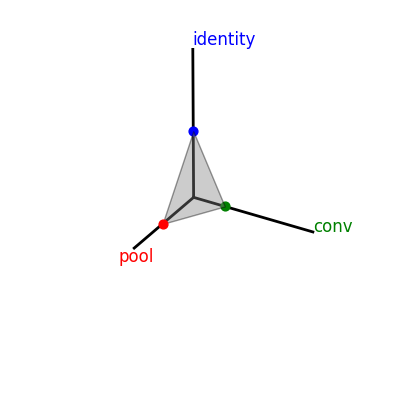
\includegraphics[width=0.32\linewidth]{graf_1.png}\hfill
    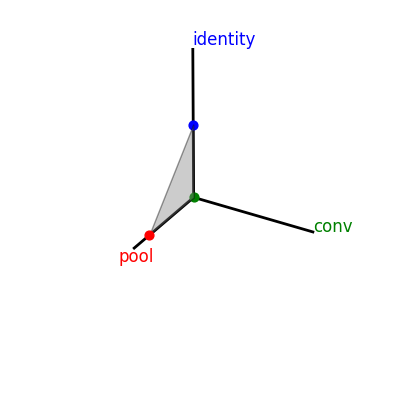
\includegraphics[width=0.32\linewidth]{graf_2.png}\hfill
    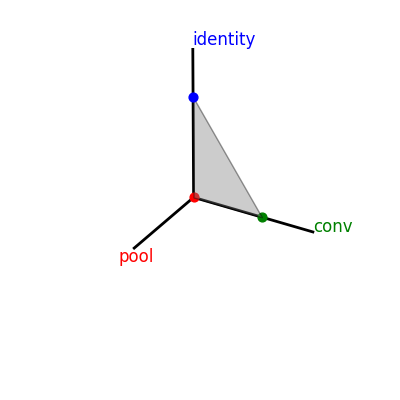
\includegraphics[width=0.32\linewidth]{graf_3.png}
    \caption{Operation statistics of the three sampled
    architectures: \textbf{(A)} uniform regularisation,
    \textbf{(B)} heavy penalty on convolutions,
    \textbf{(C)} heavy penalty on pooling.}
    \label{fig:operation-distribution}
\end{figure}

\begin{table}[!ht]
    \centering
    \caption{Quantitative comparison of the sampled architectures.}
    \label{tab:quantitative-results}
    \begin{tabular}{lccc}
        \hline
        & (A) uniform & (B) conv.\ penalty & (C) pool.\ penalty \\[2pt] \hline
        Test accuracy [\%]           & 82.5 & 79.2 & \textbf{85.0} \\
        Parameter count              & 38\,304 & \textbf{5\,120} & 143\,488 \\
        \# Pooling layers            & 12 & 17 & \textbf{0} \\
        \# Convolution layers        & 6  & \textbf{0} & 13 \\
        \# Identity connections      & 10 & 11 & 15 \\\hline
    \end{tabular}
\end{table}

Figure~\ref{fig:operation-distribution} visualises how the choice of the complexity vector shapes the architecture, while
Table~\ref{tab:quantitative-results} reports key quantitative metrics.
Several observations stand out:

\begin{itemize}
    \item \textbf{Controllable complexity.}  
    Penalising convolutions (profile B) eliminates them entirely, resulting in    an ultra-compact model with only 5k parameters.
    Conversely, penalising pooling (profile C) encourages the hypernetwork
    to favour convolutions, increasing both parameter count and accuracy.
    \item \textbf{Accuracy–latency trade-off.}  
    Although profile B sacrifices 3.3 pp of accuracy relative to the baseline
    (A), it reduces the number of MAC-intensive operations and therefore the
    expected latency—highly desirable for edge devices.
    \item \textbf{Single training run.}  
    All three architectures originate from the \emph{same} trained
    hypernetwork; no additional architecture search is required when the
    hardware budget changes.
\end{itemize}

These results confirm that the proposed single-level, hardware-aware NAS framework enables fine-grained control over model complexity without compromising search efficiency.


\section{Conclusion}


We have presented a unified neural architecture search framework that
combines a simplex-based complexity vector,
a latency-aware objective inspired by FBNet, and
hypernetwork-driven Gumbel–Softmax sampling.
Unlike bilevel DARTS, our formulation trains weights and structure in a singleloop, dramatically simplifying optimisation.



\section{NEW: Problem Statement}

\subsection{Hardware-aware formulation}

Let $\mathfrak D=\{(x_i,y_i)\}_{i=1}^{\mathcal N}$ be a classification dataset with inputs $x_i\in\mathbf X$ and labels $y_i\in\mathbf Y$.  
Our goal is to discover a neural architecture that attains high predictive accuracy and satisfies hardware constraints—most notably the end-to-end inference latency on a target device. We follow the latency–driven design philosophy of FBNet \cite{Wu_2019_CVPR}, where \textit{measured} operation delays are used instead of proxy metrics such as FLOPs.

\subsection{Hypernetwork–driven search space}

As in differentiable NAS, a candidate network is assembled from repeated \emph{cells} whose internal connectivity is fixed while the operation on each edge is chosen from a finite set $\mathcal G=\{g^{(1)},\dots,g^{(k)}\}$.  
Instead of learning a separate set of continuous mixing coefficients for every edge, we generate them with a \emph{hypernetwork} \cite{yakovlev2021neural}.  
Concretely, let  
\[
\mathbf S\in\Delta^{k-1}\;=\;\bigl\{\mathbf S\in\mathbb R^{k}\,\bigl|\,\sum_{j=1}^kS_j=1,\,S_j\!\ge\!0\bigr\}
\]
be a \textbf{complexity vector} sampled once per mini-batch from the uniform distribution over the simplex.  
A learnable hypernetwork $H_{\boldsymbol a}\colon\Delta^{k-1}\to\mathbb R^{?}$, parameterised by $\boldsymbol a$, maps $\mathbf S$ to the matrix of \emph{logits} $\boldsymbol\alpha=H_{\boldsymbol a}(\mathbf S)$, one $k$-dimensional row per edge $(i,j)$.

For every edge we draw a one-hot vector
\[
\boldsymbol\gamma_{(i,j)}\sim\text{Gumbel–Softmax}\bigl(\boldsymbol\alpha_{(i,j)},t\bigr),
\]
so that edge $(i,j)$ executes operation 
$g_{(i,j)}( \cdot )=\sum_{m=1}^k\gamma^{(m)}_{(i,j)}\,g^{(m)}(\cdot)$.
The temperature~$t$ is annealed during training, gradually turning the relaxed architecture into a discrete one.

\subsection{Single-level objective}

Each primitive $g^{(m)}$ is associated with a measured latency $L^{(m)}$ on the target hardware; the latency of a sampled architecture $\boldsymbol\gamma$ is  
$
\operatorname{Latency}(\boldsymbol\gamma)=\sum_{(i,j)\in\mathcal E}\sum_{m=1}^{k}\gamma^{(m)}_{(i,j)}\,L^{(m)}.
$
We jointly learn network weights $\boldsymbol w$ and hypernetwork parameters $\boldsymbol a$ by minimising a \emph{single-level} loss:
\[
\min_{\boldsymbol w,\boldsymbol a}\;
\mathbb E_{\mathbf S\sim\mathcal U(\Delta^{k-1})}
\;\mathbb E_{\boldsymbol\gamma\sim\mathrm{GS}(H_{\boldsymbol a}(\mathbf S),t)}
\Bigl[\,\mathcal L_{\text{task}}(\boldsymbol w,\boldsymbol\gamma)\;
+\;\kappa\,\operatorname{Latency}(\boldsymbol\gamma)\Bigr],
\]
where $\mathcal L_{\text{task}}$ is the cross-entropy loss on the training data and $\kappa>0$ controls the accuracy–latency trade-off.



% теорема

\bibliographystyle{plain}
\bibliography{sample}

\end{document}